
\documentclass[aspectratio=169]{beamer}
\usepackage[utf8]{inputenc}
\usepackage[T1]{fontenc}
%%%%%%%
% \usepackage{layout}
% \usepackage{lipsum}
%%%%%%%
\usetheme[% Complete settings. Default value in []
% titleimagecolor=red,       % [gray], darkgray, red, blue, green
% titleimagemargin=2mm,      % Distance [2mm]    Frame around title page image
% navigationsymbols=false,   % true   / [false]  Navigation symbols in the foot
% mathseriffont=false,       % true   / [false]  Serif / non-serif math fonts
% foot=true,                 % [true] / false    Footline or not
% nofootslidenum=false       % true   / [false]  Keep slide num even when foot=false
% footlogo=true,             % [true] / false    Put LU logo to the left of footer
% english=true,              % [true] / false    English / Swedish logo
% LTHlogo=false,             % true   / [false]  Use LTH logo instead of LU on title and end pages.
% blackenumeratenumber=true, % [true] / false    Black enumerate numbers, o.w. Lund bronze
% blackitemmark=false,       % true   / [false]  Black item marks, o.w. Lund bronze
% defaultfont=false,         % true   / [false]  Falls back to default beamer fonts
% sectionframe=true,
]{ulund}
%%%%%%%%%%%%%%%%%%%%% Layout commands 
%%%% Foot
% \ulundfootleft{\insertshortauthor}
% \ulundfootmid{\insertshorttitle}
% \ulundfootright{\insertframenumber}% {\insertframenumber:\inserttotalframenumber}
%%%% Titleimage
\titleimage{Pictures/ULUNDcolor} % Replaces the LU image. Voids option titleimagecolor
%%%%%%%%%%%%%%%%%%%%%%%%%%%%%%%%%%%
\title[Scala First Lessons]{Scala First: \vspace{0.25em}\newline \fontsize{16}{25}\selectfont Lessons from 3 student generations }
\author[Bjorn Regnell]{%
  Bjorn Regnell\newline
  Dept.\@ of Computer Science, Lund University}
%%%%%%%%%%%%%%%%%%%%%
%\usepackage{verbatim}
%%%%%%%%%%%%% Verbatim code box
\usepackage[skins,listings]{tcolorbox}
\tcbuselibrary{listingsutf8}

\begin{document}
\begin{frame}[plain]% Use plain to suppress footline box
  \titlepage
\end{frame}%

%%%%%%%%%%%%%%%
\begin{frame}[fragile]
  \frametitle{Scala First Lessons}
Agenda:
\begin{itemize}
\item Why Scala First?
%Why did we introduce Scala as a first language for computer science and engineering students at Lund Univ.?
\item Implementing Scala first @ Lund University 
%\item How to handle mixed programming pre-knowledge?
%How did we deal with a very broad spectrum of pre-knowledge in programming?
%\item How to develop teaching resources for Scala first?
%How did we bootstrap our open source teaching resources?
%\item How to design a progression for Scala first?
%What are the difficult trade-offs when designing a coherent progression in beginner programming in Scala?
%\item How to balance OO and FP? %How did we balance OO and FP in Scala first?
\item What did we learn?
%\item Benefits and pitfalls of Scala first?
%\item What did we learn after 3 generations of beginner students?
\item The road ahead%What is the road ahead for Scala at Lund University?
\end{itemize}
\end{frame}

\titleimagecolor{red}
\section{Why Scala First?}



\begin{frame}[plain]
\begin{figure}
\centering
\begin{tikzpicture}[overlay] 
\node [] at (0.0mm,-15.0mm) {%
  \includegraphics[height=1.2\paperheight]{Pictures/kids-programming}%
};
\end{tikzpicture}%
\end{figure}%
\end{frame}%


\begin{frame}[plain]
  \begin{figure}
  \centering
  \begin{tikzpicture}[overlay] 
  \node [] at (0.0mm,-5.0mm) {%
  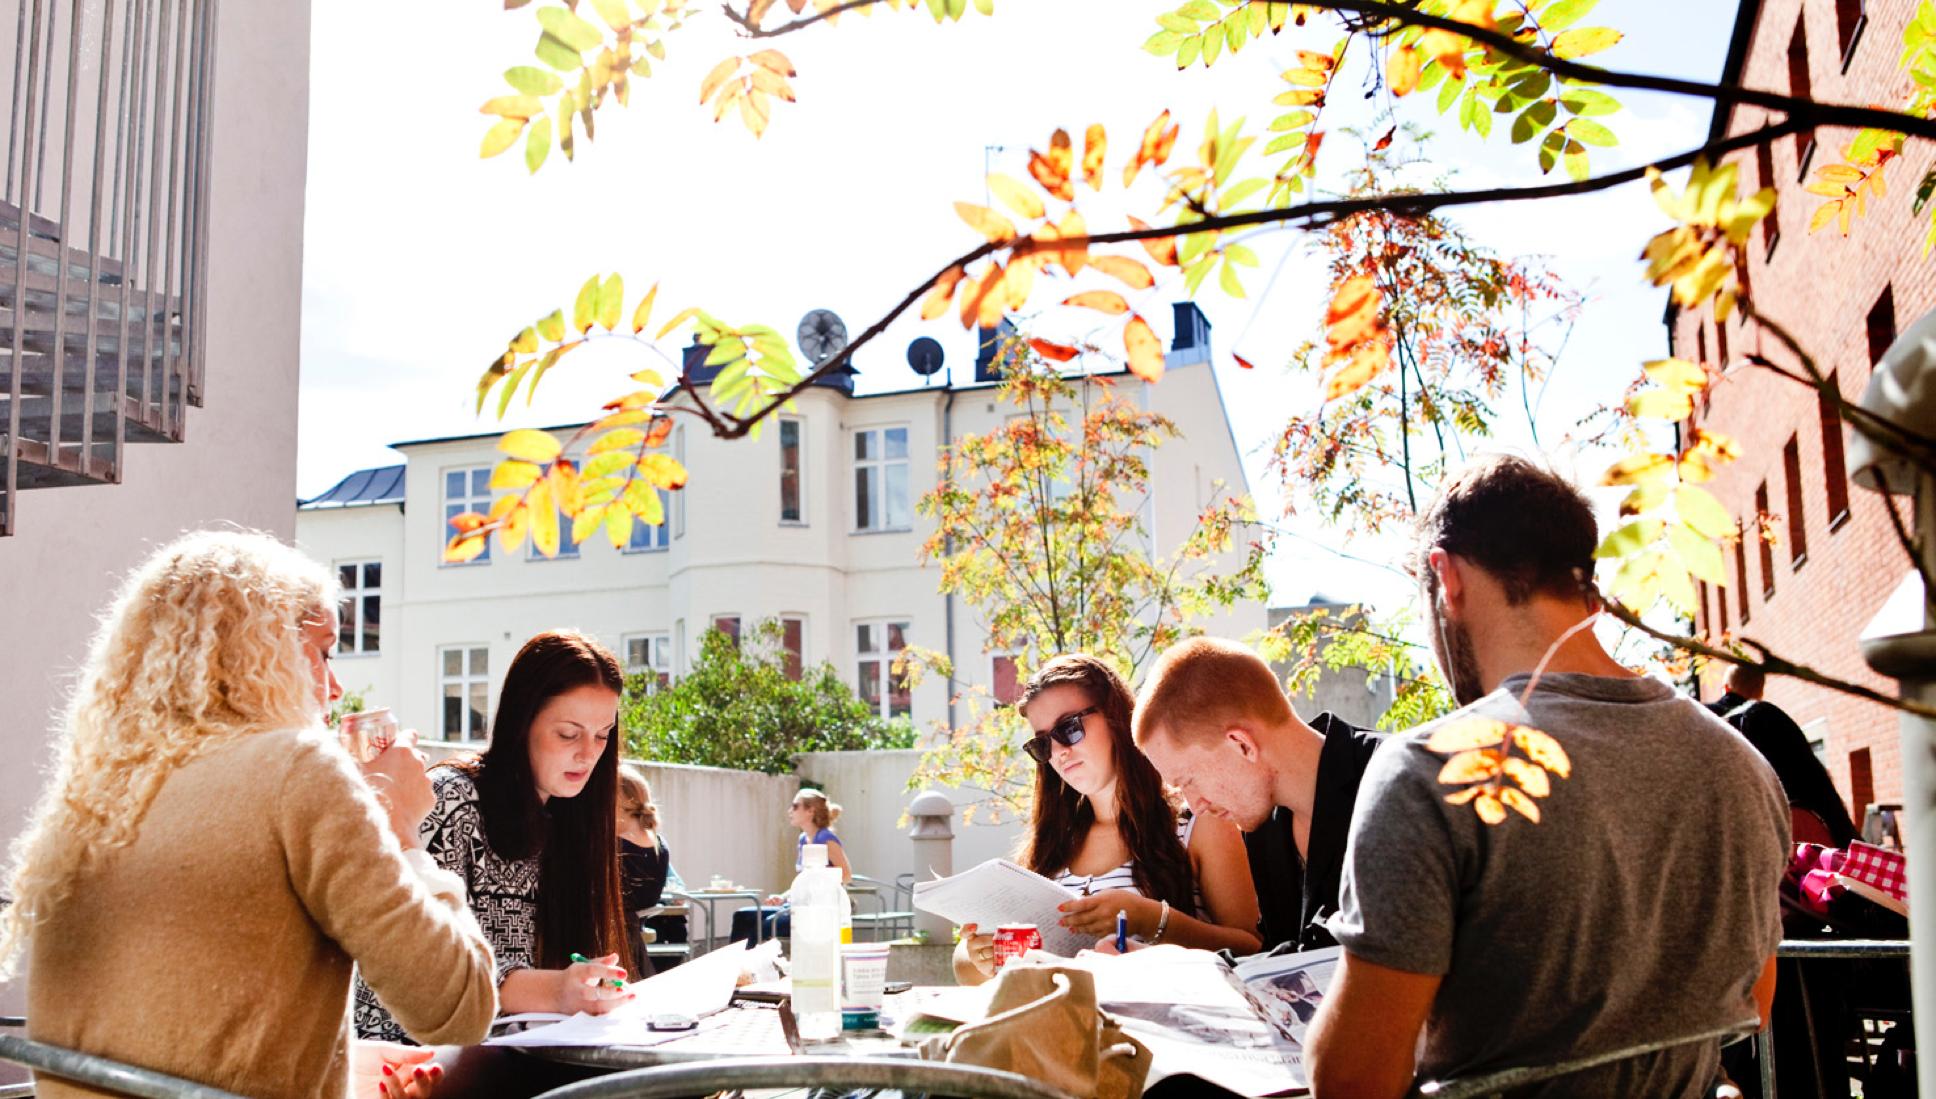
\includegraphics[height=1.2\paperheight]{Pictures/titlepictureGroup}};
  \end{tikzpicture}%
  \end{figure}%
  \end{frame}%

\begin{frame}[plain]
\endpage
\end{frame}
  
\end{document}